

Los instrumentos y materiales utilizados a lo largo de todo este trabajo práctico, son los siguientes:

\begin{itemize}
    \item Osciloscopios Digitales: marca RIGOL, modelo DS1052E; marca UNI-T, modelo UTD2102CEX.
    \item 2 Puntas de Osciloscopio Hantek de 100 Mhz.
    \item Generador de funciones: marca GW INSTEK, modelo GFG 3015.
    \item Multímetro digital marca UNI-T, modelo UT890C.
    \item Fuente de tensión variable del laboratorio central de la UTN-FRC.
    \item Kit del TP2 de Medidas Electrónicas (disponible en el laboratorio central de electrónica de la UTN-FRC). Contiene una fuente con salida regulada y no regulada de aprox 12V; un circuito generador de una onda de aprox. 400 Hz; un marcador de teléfono antiguo (disco) con un circuito incorporado para poder ver las señales; y una placa auxiliar para generar un tren de pulsos diferencial.
    
\end{itemize}


%Poner las placas del kit con fotos y explicar un poco y poner el numero de kit

Además de los instrumentos de medición y fuentes de alimentación, en este práctico se trabajará con dos circuitos auxiliares. Ambos circuitos son amplificadores (sin una aplicación específica), pero el segundo circuito tiene la posibilidad de realimentación.

\subsection{Circuito Amplificador 1}
\label{sec:Amp1}

El primer circuito amplificador que se empleará, consta de dos placas, una para el amplificador y otra que es un circuito auxiliar, ya preparado para que se puedan realizar las mediciones de las señales de entrada y salida, y de impedancia (también de entrada y salida), mediante unas resistencias variables. Este kit es el que se muestra en la figura \ref{fig:DUT}. 

%Imagen doble del circuito y circuito real

\begin{figure}[H]
    \begin{center}
        \begin{subfigure}[b]{0.5\textwidth}
        \centering  
            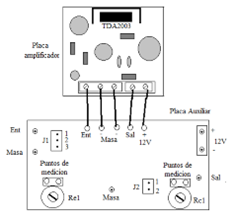
\includegraphics[width=0.8\textwidth]{Imagenes/placa1.png}
        \caption{Diagrama de las placas}
        \label{fig:placa1}
    \end{subfigure}
    \hfill
    \begin{subfigure}[b]{0.49\textwidth}
        \centering
            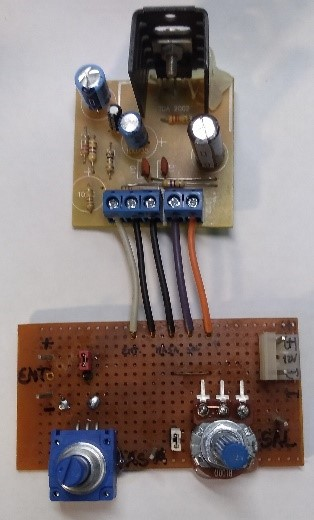
\includegraphics[width=0.5\textwidth]{Imagenes/placa1b.jpg}
        \caption{Placas reales}
        \label{fig:placa1b}
    \end{subfigure}
    \caption{Vistas de las placas amplificadora y auxiliar}
    \label{fig:DUT}
    \end{center}
\end{figure}

El circuito de la placa amplificadora (placa superior de la figura \ref{fig:placa1}), es el que se muestra a continuación en la figura \ref{fig:amp1}.

%Imagen circuito amplif

\begin{figure}[H]
    \centering
    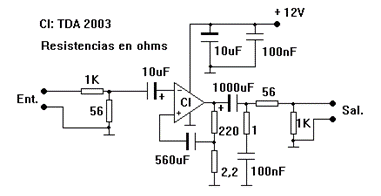
\includegraphics[width=0.68\linewidth]{Imagenes/amp1.png}
    \caption{Esquemático placa amplificadora}
    \label{fig:amp1}
\end{figure}

Este conjunto de placas se encuentra disponible en el pañol del laboratorio central de la Universidad Tecnológica Nacional, Facultad Regional Córdoba. Se puede pedir bajo el nombre de circuito amplificador para el trabajo práctico 3 de la materia \textit{Medidas Electrónicas I}. 

Cabe destacar que las placas disponibles en el laboratorio están numeradas para en caso de necesitar utilizarlas en días diferentes, saber identificar el mismo conjunto y que las mediciones sean certeras. 

En nuestro caso, se utilizó el conjunto de placas número \textbf{2}.

\begin{table}[H]
    \centering
    \begin{tabular}{|c|c|}
        \hline
            Conjunto &  \\
            de Placas & 2 \\
            Nro: & \\
        \hline
    \end{tabular}
    \def\tablename{Tabla} 
    \caption{Conjunto de placas bajo ensayo utilizado}
    \label{tab:DUT}
\end{table}

Por último, se muestra una imagen del circuito equivalente del amplificador a ensayar y los valores nominales de algunas de las magnitudes que se medirán.

\begin{figure}[H]
    \centering
    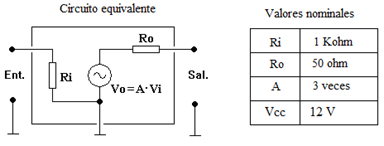
\includegraphics[width=0.7\linewidth]{Imagenes/amp1circeq.png}
    \caption{Circuito equivalente y valores nominales del amplificador}
    \label{fig:amp1circeq}
\end{figure}




\subsection{Circuito Amplificador 2 (posibilidad de realimentación)}
\label{sec:Amp2}

El segundo amplificador a utilizar, consiste en un amplificador con realimentación que se encuentra ya preparado en el laboratorio central de electrónica.

El esquema del amplificador utilizado es el siguiente:

\begin{figure}[H]
    \centering
    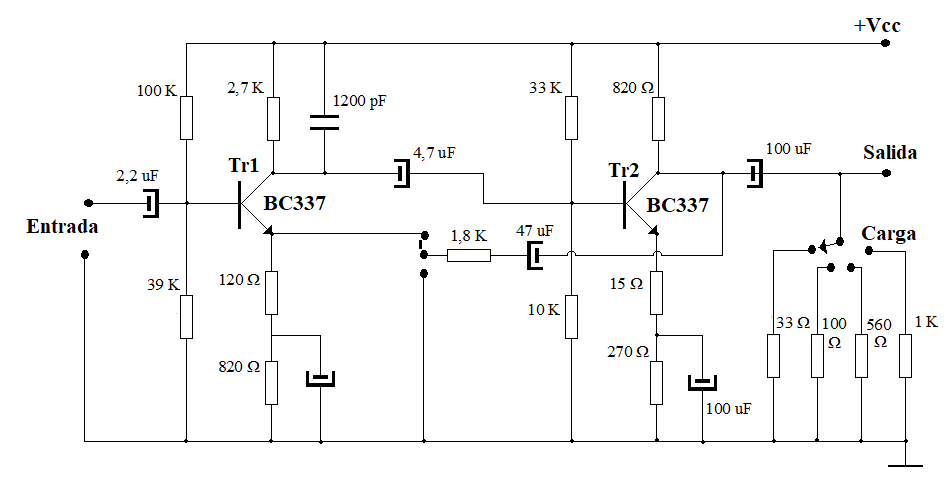
\includegraphics[width=\textwidth]{Imagenes/Esq_amp_tp3.png}
    \caption{Amplificador realimentado}
    \label{fig:esq_amp_tp3}
\end{figure}

\begin{figure}[H]
    \centering
    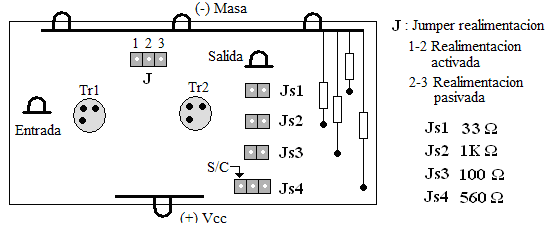
\includegraphics[width=0.8\textwidth]{Imagenes/Esq2_amp_tp3.png}
    \caption{Amplificador realimentado}
    \label{fig:esq2_amp_tp3}
\end{figure}


Este amplificador consta de 4 resistencias a las salidas de diferentes valores(1~k\ohm, 560~\ohm, 100~\ohm~y 33~\ohm), las cuales se pueden seleccionar con el jumper \textbf{Js} para que sea nuestra carga.

El Jumper \textbf{J} le permitirá activar o pasivar el lazo de realimentación. El amplificador está preparado para alimentarse con una tensión continua de +12V y tanto la salida como la entrada están acopladas en CA.


